The planning and development of the installation of toothbrush production line in the eco-city of Taijin in China is guided by a comprehensive set of Key Performance Indicators (KPIs) covering its ecological, economic and social development.\\

There are seven quantitatives and three qualitatives KPIs.

\subsection{Quantitatives KPIs}

\subsubsection{Developing a Dynamic and Efficient Economy}
\begin{description}
    \item[Use of renewable resources]: using recycled resources to save money by 40\%.
    \item[Control the production]: Production control to avoid overproduction, which can be costly in terms of storage and resources.
    \item[Transportation]: Use intelligent way of transportation in order to save mony by 60\%.
    \item[Client satisfaction]: Gather user feedback to improve the product.
\end{description}

\subsubsection{Developing efficient machines}
\begin{description}
    \item[Maintenance machine]: machines must be operational at least 99\% of the time.
    \item[Cleaning machine]: the machines must not know any dirt that may impact the quality of the product.
\end{description}

\subsubsection{Developing efficient employers}
\begin{description}
    \item[Formation]: In order to improve the quality and productivity of employees by 70\%.
\end{description}

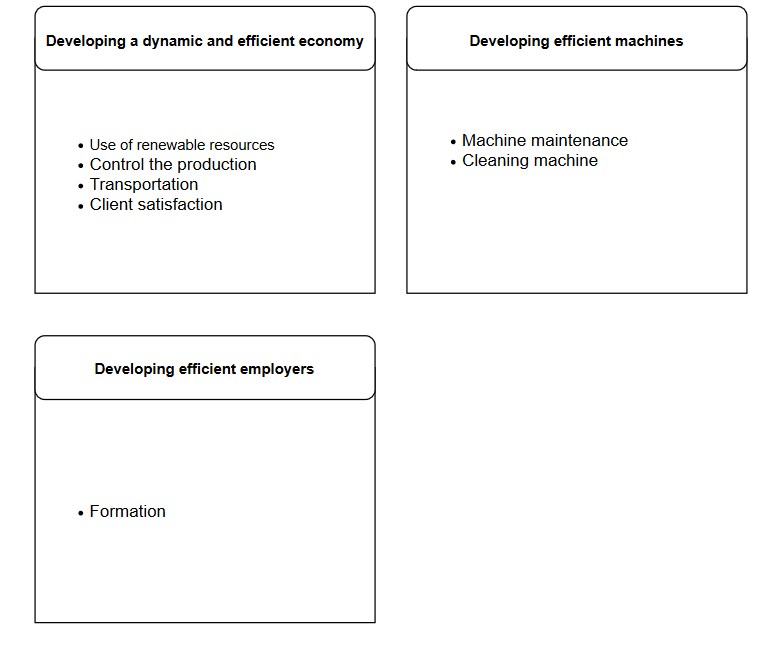
\includegraphics{Img/tableaudebord.png}

\subsubsection{Qualitative KPIs}
\begin{itemize}
    \item Maintain quality and safe production through careful monitoring of machines and production.
    \item Adopt safety policies for employees that will promote their well-being and the smooth running of production.
    \item Maintain the most eco-responsible production line by following the environmental standards in the factory.
\end{itemize}

